\documentclass[oneside]{article}
\usepackage{wallpaper}
\usepackage{geometry}
\usepackage{xeCJK}  % 支援中文
\setCJKmainfont{a.otf}
\usepackage[
    unicode=true,
    bookmarks=true,
    bookmarksnumbered=false,
    bookmarksopen=true,
    bookmarksopenlevel=1,
    breaklinks=false,
    pdfborder={0 0 0},
    backref=false,
    colorlinks=false
    ]{hyperref}
\usepackage{lastpage}
\usepackage{hyphenat}
\usepackage{hyphsubst}
\usepackage{tabularx}
\usepackage{moresize}
\usepackage[document]{ragged2e}
\usepackage[scaled]{helvet}
\usepackage{fontawesome5}
\usepackage[defaultfam,tabular,oldstyle]{montserrat}
\usepackage[T1]{fontenc}
\renewcommand*\oldstylenums[1]{{\fontfamily{Montserrat-TOsF}\selectfont #1}}
\usepackage{titlesec}
\usepackage{xcolor}
\usepackage{tikz}
\setlength{\parindent}{0pt}
\titleformat{\section}{\normalfont}{}{0pt}{}
\renewcommand{\arraystretch}{1.4}
\setlength\fboxrule{0pt}
\setlength\fboxsep{12pt}
\renewcommand{\baselinestretch}{1.1}
\titlespacing{\section}{0pt}{1.5ex plus .1ex minus .2ex}{1pc}
\newcolumntype{Y}{>{\RaggedRight\arraybackslash}X}
\hypersetup{
    pdftitle={John Doe - CV - English},
    pdfauthor={John Doe},
    pdfsubject={CV}
}
\geometry{
    a4paper,
    left=0pt,
    right=0pt,
    top=0pt,
    bottom=0pt,
    nohead,
    % includefoot,
    nomarginpar
}

% Background Color of the Sidebar Column
\definecolor{sidebg}{cmyk}{1, 0.02, 0, 0.56}
% Background Color of the Main Column
\definecolor{mainbg}{cmyk}{0, 0, 0.07, 0.04}

% Text Color of the Main Column
\definecolor{maintext}{cmyk}{1, 0.02, 0, 0.8}
% Text Color of the Sidebar Column
\definecolor{sidetext}{cmyk}{0, 0, 0.07, 0.04}

\pagecolor{mainbg}

\begin{document}
\setlength{\topskip}{0pt}\setlength{\footskip}{0pt}%
\fcolorbox{red}{sidebg}{%
    \begin{minipage}[t][\textheight-2\fboxsep-2\fboxrule][t]{\dimexpr0.40\textwidth-2\fboxrule-2\fboxsep\relax}
        \color{sidetext}
        %%%%%%%%%%%%%%%%%%%%%%%%%%%%%%%%%%%%%%%%%%%%%%%%%%%%
        % YOUR NAME, PRONOUNS, OCCUPATION(s), AND HEADSHOT
        \vspace{1cm} \\
        {\bfseries\scshape\HUGE 王子謙} \\
        \vspace{.2cm} \\
        {\bfseries\scshape\Huge Tzu-Chien Wang} \qquad {}
        \vspace{.3cm} \\
        \\
        \\
        \begin{center}
            \begin{tikzpicture}
            \clip (0,0) circle (3cm) node[anchor=center] {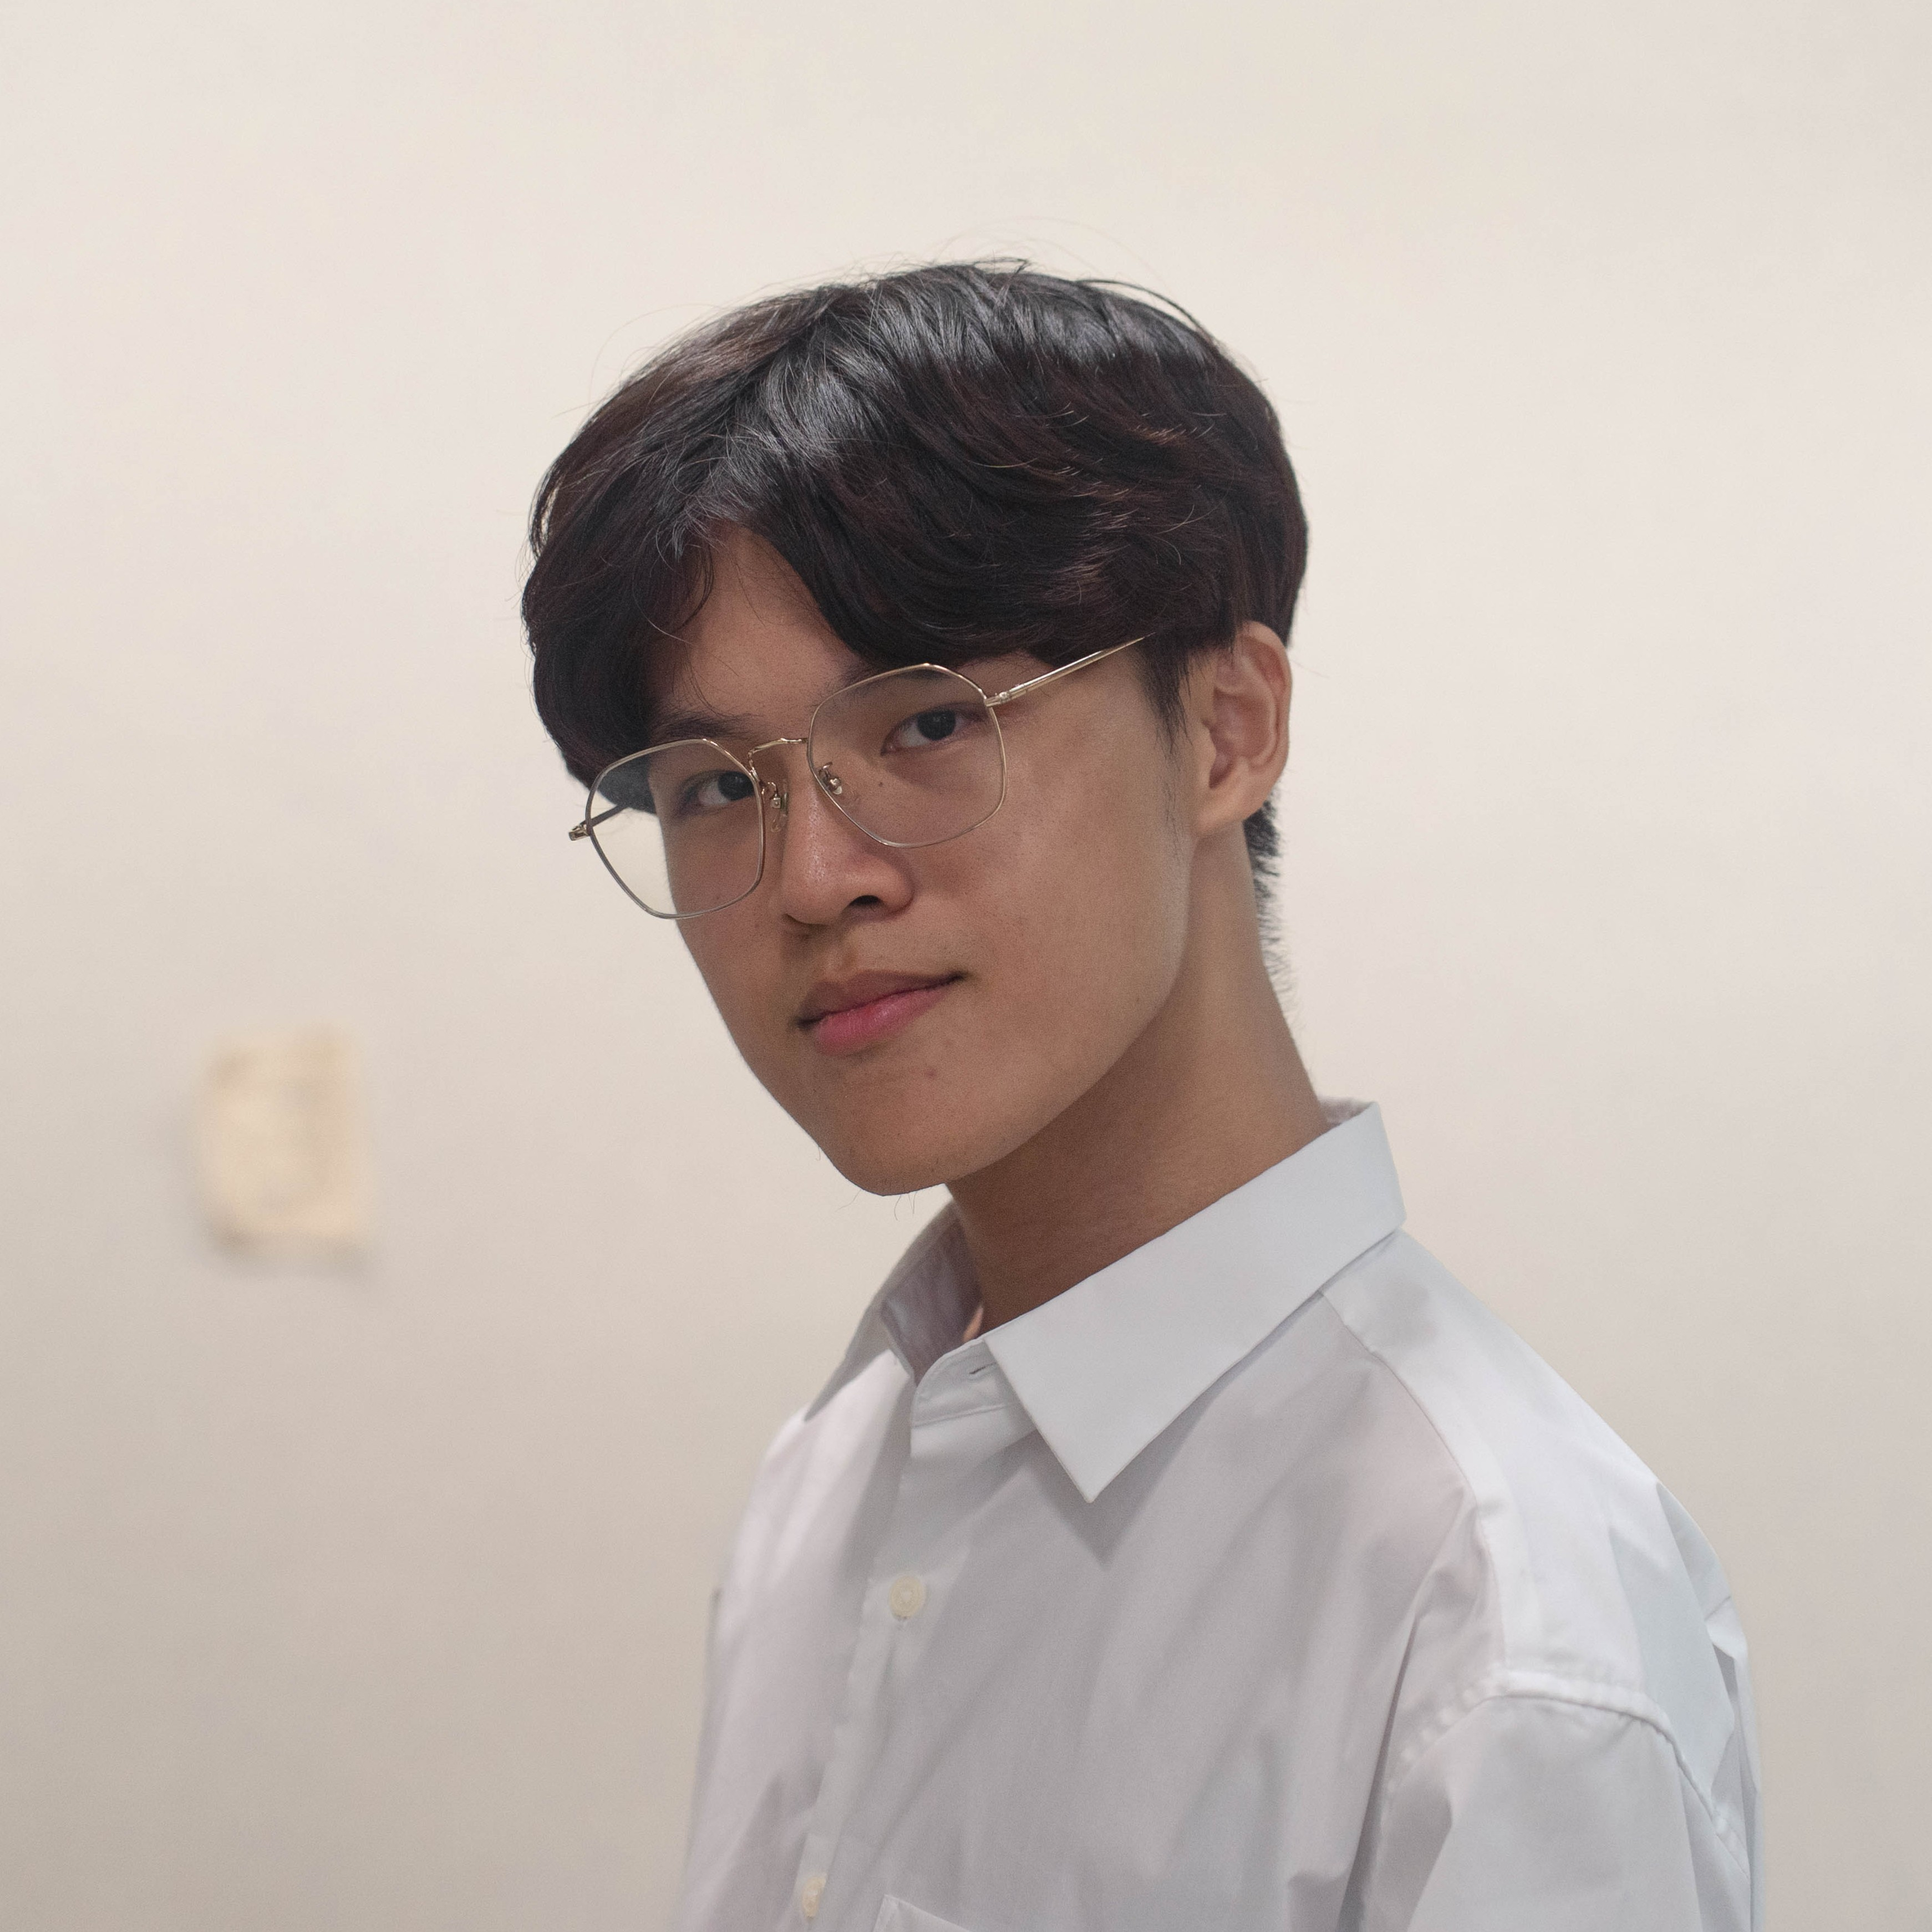
\includegraphics[width=6cm]{portait_template.jpg}}; 
            \end{tikzpicture}
        \end{center}
        \vspace{.3cm}
        %%%%%%%%%%%%%%%%%%%%%%%%%%%%%%%%%%%%%%%%%%%%%%%%%%%%
        % YOUR PERSONAL INFROMATION
        \phantomsection{}
        \addcontentsline{toc}{section}{Personal info}
        \section*{\large Personal info}
        \begin{tabularx}{\textwidth}{cY}
            \faStarOfLife{} & 03/30/2004 \\[.5ex]
            \faPhone{}      & 0979717554 \\[.5ex]
            \faMapMarker{}  & 桃園市中壢區五族二街111號6樓 \\[.5ex]
            \faEnvelope{}   & \href{mailto:wangalan1234@gmail.com}{wangalan1234@gmail.com} \\[.5ex]
            \faGithub{}     & \href{https://github.com/ddc0330}{ddc0330} \\[.5ex]
        \end{tabularx}
        \vspace{.3cm} \\
        \rule{\linewidth}{0.4pt} \\
        %%%%%%%%%%%%%%%%%%%%%%%%%%%%%%%%%%%%%%%%%%%%%%%%%%%%%%%%%
        
        % YOUR SKILLS
        % Add/Remove as seen fit, Icons: https://packages.oth-regensburg.de/ctan/fonts/fontawesome5/doc/fontawesome5.pdf
        \phantomsection{}
        \addcontentsline{toc}{section}{Skills}
        \section*{\large Skills}
        \begin{tabularx}{\textwidth}{cY}
            \faCode{}        & C++, C, Python, Assembly, JAVA, JS\\[.5ex]
            \faPen*{}        & LaTeX, HTML, CSS,  \\[.5ex]
            \faToolbox{}     & pytorch, pygame, tensorflow, yfinance\\[.5ex]
            \faCogs{}        & Linux, Windows \\[.5ex]
        \end{tabularx}
        \vspace{1pt} \\
        \rule{\linewidth}{0.4pt}
        %%%%%%%%%%%%%%%%%%%%%%%%%%%%%%%%%%%%%%%%%%%%%%%%%%%%%%%%%%%%%%%%
        % YOUR PERSONAL INFROMATION
        \phantomsection{}
        \addcontentsline{toc}{section}{Personal info}
        \section*{\large Education}
        \begin{tabularx}{\textwidth}{cY}
        $\bullet$    & \textbf{台南市國立成功大學大學部在學三年級} \\[.5ex]
        $\bullet$    & \textbf{桃園市市立武陵高中} \\[.5ex]
        \end{tabularx}
        \vspace{.3cm} \\
        %%%%%%%%%%%%%%%%%%%%%%%%%%%%%%%%%%%%%%%%%%%%%%%%%%%%%%%%%
        % GRADESCALE (if nesseary, e.g. if you apply abroad, where scales 
        % are different. You should at least provide, what the best possible
        % grade and what the worst possible grade is)
        
    \end{minipage} 
}
\hfill
\fcolorbox{red}{mainbg}{%
    \begin{minipage}[t][\dimexpr\textheight-2\fboxrule-2\fboxsep\relax][t]{\dimexpr0.6\textwidth-2\fboxrule-2\fboxsep\relax}
        \color{maintext}
        %%%%%%%%%%%%%%%%%%%%%%%%%%%%%%%%%%%%%%%%%%%%%%%%%%%%%%%%%%
        % ABOUT ME
        \vspace{1.5cm} \\
        \phantomsection{}
        \addcontentsline{toc}{section}{About Me}
        \section*{\scshape\Huge About Me \rule{\linewidth}{0.4pt}}
        
        \Large 你好,我是王子謙,成大資訊工程學系大三在學生。我對於資訊工程有著巨大熱忱,因為資訊工程的強大能幫助我解決生活中的問題,如:幫助我快速輸入驗證碼、預測股票等...,更能夠幫助我實現靈感,如:我正在製作一個幫助人們色彩分析的 AI。
        
        \bigskip

        課餘期間,我積極參與校園中的各大活動,藉此培養我的團隊合作、溝通能力,也更加了解到自己擁有在一個團隊中擔任領導者的特質。

        \bigskip

        在做專題的過程中,我也清楚認知到自己對資訊工程知識的欠缺,因此,暑期實習或是工作中,我期望學習到更多資訊工程相關技術與知識,並帶給公司最大的利益。
        
         \\
        \vspace{.5cm} \\

        
        %%%%%%%%%%%%%%%%%%%%%%%%%%%%%%%%%%%%%%%%%%%%%%%%%%%%%%%%%%%
        % EDUCATION
        \phantomsection{}
        \addcontentsline{toc}{section}{Education}
        \section*{\scshape\Huge Experience \rule{\linewidth}{0.4pt}}
%
        {\Large \textbf{Projects}} \\[1ex]
        {$\bullet$ & 專題研究:股價預測與市場恐慌指數} \\[1ex]
        {$\bullet$ & 專題研究:AI韓式色彩分析(製作中)} \\
        {\footnotesize \qquad Project link: https://coloranalysis.fun/} \\[1ex]
        {$\bullet$ & 成大課程github作品集} \\
        {\footnotesize \qquad 內容包含:程式設計作業、asembly編寫夾娃娃機、java遊戲製作等...} \\[2ex]
        {\Large \textbf{Extracurricular Activities}} \\[1ex]
        {$\bullet$ & 資工系系學會副會長(大二)} \\[1ex]
        {$\bullet$ & 桃友會會長(大二)} \\[1ex]
        {$\bullet$ & 積極參與系外活動} \\
        {\footnotesize \qquad 曾擔任校園舞會副召集人、成大單車節行銷部工人、桃友會返鄉服務志工} \\[1ex]
        {$\bullet$ & 積極參與系上活動} \\
        {\footnotesize \qquad 協助籌辦迎新、表演活動、與教授們商討系上事宜等...} \\[2ex]
         %%%%%%%%%%%%%%%%%%%%%%%%%%%%%%%%%%%%%%%%%%%%%%%%%%%%%%%%%%%
    \end{minipage}
}%
\end{document}